\documentclass[master, och, pract]{SCWorks}
% Тип обучения (одно из значений):
%    bachelor   - бакалавриат (по умолчанию)
%    spec       - специальность
%    master     - магистратура
% Форма обучения (одно из значений):
%    och        - очное (по умолчанию)
%    zaoch      - заочное
% Тип работы (одно из значений):
%    coursework - курсовая работа (по умолчанию)
%    referat    - реферат
%    otchet     - универсальный отчет
%    nirjournal - журнал НИР
%    diploma    - дипломная работа
%    pract      - отчет о научно-исследовательской работе
%    autoref    - автореферат выпускной работы
%    assignment - задание на выпускную квалификационную работу
%    review     - отзыв руководителя
%    critique   - рецензия на выпускную работу
% Включение шрифта
%    times      - включение шрифта Times New Roman (если установлен)
%                 по умолчанию выключен
\usepackage{preamble}

\begin{document}

% Кафедра (в родительном падеже)
\chair{Информатики и программирования}

% Тема работы
\title{Разработка платформы единого резюме}

% Курс
\course{2}

% Группа
\group{273}

% Факультет (в родительном падеже) (по умолчанию "факультета КНиИТ")
% \department{факультета КНиИТ}

% Специальность/направление код - наименование
% \napravlenie{02.03.02 "--- Фундаментальная информатика и информационные технологии}
\napravlenie{02.04.03 "--- Математическое обеспечение и администрирование информационных систем}
% \napravlenie{09.03.01 "--- Информатика и вычислительная техника}
% \napravlenie{09.03.04 "--- Программная инженерия}
% \napravlenie{10.05.01 "--- Компьютерная безопасность}

% Для студентки. Для работы студента следующая команда не нужна.
% \studenttitle{Студентки}

% Фамилия, имя, отчество в родительном падеже
\author{Кулакова Максима Сергеевича}

% Руководитель НИР
\nirtitle{к.\,э.\,н., доцент} % степень, звание
\nirname{Л.\,В.\,Кабанова}

% Заведующий кафедрой
\chtitle{к.\,ф.-м.\,н.} % степень, звание
\chname{М.\,В.\,Огнева}

% Научный руководитель (для реферата преподаватель проверяющий работу)
\satitle{к.\,э.\,н., доцент} %должность, степень, звание
\saname{Л.\,В.\,Кабанова}

% Руководитель практики от организации (только для практики, для остальных типов
% работ не используется)
\patitle{к.\,э.\,н., доцент}
\paname{Л.\,В.\,Кабанова}

% Семестр (только для практики, для остальных типов работ не используется)
\term{1}

% Наименование практики (только для практики, для остальных типов работ не
% используется)
\practtype{производственная (научно-исследовательская работа)}

% Продолжительность практики (количество недель) (только для практики, для
% остальных типов работ не используется)
\duration{18}

% Даты начала и окончания практики (только для практики, для остальных типов
% работ не используется)
\practStart{01.09.2023}
\practFinish{14.01.2024}

% Год выполнения отчета
\date{2023}

\maketitle

% Включение нумерации рисунков, формул и таблиц по разделам (по умолчанию -
% нумерация сквозная) (допускается оба вида нумерации)
\secNumbering

\tableofcontents

% Раздел "Обозначения и сокращения". Может отсутствовать в работе
% \abbreviations
% \begin{description}
%     \item ... "--- ...
%     \item ... "--- ...
% \end{description}

% Раздел "Определения". Может отсутствовать в работе
% \definitions

% Раздел "Определения, обозначения и сокращения". Может отсутствовать в работе.
% Если присутствует, то заменяет собой разделы "Обозначения и сокращения" и
% "Определения"
% \defabbr

% Ссылка на источник в тексте
% \cite{}

\intro
Вопрос поиска работы всегда находился перед лицом человека, ведь работа должна 
приносить не только деньги, но и удовлетворение физических и психологических 
потребностей человека. Наиболее актуальной проблемой со стороны соискателя является 
то, где искать необходимого ему работодателя, а также с какой стороны преподнести 
свои навыки и умения, чтобы в ближайшие дни занимать рабочее место своей мечты.


Задачами работы являются следующие пункты:
\begin{enumerate}
    \item Масштабирование платформы до клиент-серверного приложения;
    \item Конфигурация основного функционала; 
    \item Реализация взаимодействия по API.

    \item Обзор научной литературы (в том числе научно-технической) по теме 
    <<Разработка платформы единого резюме>>;
    \item Рассмотрение и анализ существующих платформ для создания резюме;
    \item Формулировка собственных методов разработки единой платформы резюме;
    \item Подведение итогов проведенной научно-исследовательской работы.
\end{enumerate}


% После введения — серии \section, \subsection и т.д.
\newpage
\section{Анализ научной литературы}
Рассматриваемая литература будет затрагивать тему аспектов составления резюме, 
принципы их составления и критерии, по которым работодателю с наибольшей вероятностью 
понравится грамотно составленное резюме. После проведения анализа данной темы нам 
предоставится возможность выделить основные пункты, которые будут учитываться 
при разработке собственной единой платформе резюме.

Для начала стоит рассмотреть научные статьи, связанные с доказательством важности 
правильного составления резюме в настоящее время, и какие изменения  оно претерпевает. 
В статье К.В. Косолаповой <<Типологические особенности современного резюме на английском 
языке>> автор выделяет основные пункты в резюме, которые было принято считать достаточными:
\begin{enumerate}
    \item Полные ФИО;
    \item Возраст;
    \item Место проживания на текущий момент;
    \item Место учёбы, уровень образования;
    \item Список умений;
    \item Опыт работы (при его наличии);
    \item Контактные данные.\cite{Gridneva_2021}
\end{enumerate}














\section{Реализация платформы единого резюме}
\subsection{Общие настройки динамического приложения}
Для компенсации недостатков статических сайтов и динамической генерации страниц из набора входящих параметров и данных инициализируем проект с NextJS и добавим интерфейсную библиотеку NextUI для удобства разработки следующими командами:
\begin{minted}[fontsize=\small, breaklines=true, style=bw, linenos]{bash}
npx create-next-app@latest
npm i @nextui-org/react framer-motion
\end{minted}

Для безопасной работы с проектом необходимо создать файл process.env, в котором будут хранится переменные окружения, например токен доступа к системе.

Дополнительно для каждой страницы необходимо задать общий шаблон в файле layout.tsx, находящимся в корневой папке приложения. Данная структура представляет из себя обёртку над стандартным представлением HTML файла, внутрь которого добавлено реактивное представление. Дополнительно внутри атрибутов указываются стили для блоков, такие как минимальная высота контейнера, цвет фона, размеры контейнеров, отступов и их поведение, выбор шрифта и текущая цветовая схема. В дальнейшем содержимое атрибутов className будет  игнорироваться. 
\begin{minted}[fontsize=\small, breaklines=true, style=bw, linenos]{text}
export default function RootLayout({ children, }:{
	children: React.ReactNode;
}) { return (
<html lang="en" suppressHydrationWarning>  
    <head></head>
    <body className={clsx( "min-h-screen bg-background font-sans antialiased", fontSans.variable )}>
    <Providers themeProps={{ attribute: "class", defaultTheme: "dark" }}>
    <div className="relative flex flex-col h-screen">
    <Navbar/>
    <main className="container mx-auto max-w-7xl pt-16 px-6 flex-grow">
    {children}
    </main></div></Providers></body>
</html>
);}
\end{minted}




\subsection{Написание механизма авторизации}
Для реализации авторизации создадим файл auth.ts, в котором укажем конфигурацию с сервисом Github посредством открытого протокола безопасности OAuth и с классической проверкой логина и пароля. Для этого создадим два соответсвующих свойства и в первое передадим переменные приложения для авторизации через сторонний сервис, а в втором реализуем проверку введённых в поля данных и в случае соответсвия вернём самого пользователя с его именем, фотографией профиля и ролью.
\begin{minted}[fontsize=\small, breaklines=true, style=bw, linenos]{text}
export const authConfig: AuthOptions = { providers: [
    GithubProvider({
        clientId: process.env.GITHUB_ID!,
        clientSecret: process.env.GITHUB_SECRET!,}),
    Credentials({
    credentials: {
        email: { label: 'email', type: 'email', required: true },
        password: { label: 'password', type: 'password', required: true }, },
        async authorize(credentials) {
        if (!credentials?.email || !credentials.password) return null;
        const currentUser = users.find(user => user.email === credentials.email)
        if (currentUser && currentUser.password === credentials.password) {
            const { password, ...userWithoutPass } = currentUser;
            return userWithoutPass as User;}
    return null }})
    ], pages: { signIn: '/signin' } }
\end{minted}

Ограниченик доступа неавторизованного пользователя к внутренним страницам достигается созданием файла middleware.ts, в котором через параметры указываются пути навигации и, в случае попадания в заданный путь, перевод клиента на страницу signIn.
\begin{minted}[fontsize=\small, breaklines=true, style=bw, linenos]{text}
export const config = { matcher: ['/profile/:path*', '/hh', '/resume','/protected/:path*'] }
\end{minted}

Дополнительно к предыдущему пунту контроля доступа опишем корневой файл providers.tsx, созданный для окружения корневого элемента страницы в её компоненты, свойства стилей и сессию пользователя.
\begin{minted}[fontsize=\small, breaklines=true, style=bw, linenos]{text}
export function Providers({ children, themeProps }: ProvidersProps) {
return (
<SessionProvider><NextUIProvider>
    <NextThemesProvider {...themeProps}>
        {children}
    <NextThemesProvider>
<NextUIProvider><SessionProvider>);}    
\end{minted}

Процесс авторизации реализуется на клентской и серверной части приложения, поэтому для корректного взаимодействия необходимо создать обработчик событий по API в динамическом маршруте [..auth]/route.tsx с следующими параметрами:
\begin{minted}[fontsize=\small, breaklines=true, style=bw, linenos]{text}
const handler = NextAuth(authConfig);
export { handler as GET, handler as POST }
\end{minted}

Реализуем форму авторизации через компонент SignInForm с двумя текстовыми формами, для этого
инициализируем роутер переходов, обратные вызовы для динамического контента и обработчик нажатия кнопки отправки формы, получающий данные полей и выполняющий вход в систему.
\begin{minted}[fontsize=\small, breaklines=true, style=bw, linenos]{text}
const SignInForm = () => {
    const router = useRouter();
    const [isVisible, setIsVisible] = React.useState(false);
    const toggleVisibility = () => setIsVisible(!isVisible);
    const handleSubmit: FormEventHandler<HTMLFormElement> = async (event) => {
        event.preventDefault();
        const formData = new FormData(event.currentTarget);
        const res = await signIn("credentials", {
            email: formData.get("email"),
            password: formData.get("password"),
            redirect: false
\end{minted}

Кнопка авторизации через Github работает через параметры поисковой строки, получаемые в процессе возврата на страницу платформы после успешного входа на стороне внешнего сервиса.
\begin{minted}[fontsize=\small, breaklines=true, style=bw, linenos]{text}
export const GithubButton = () => {
const searchParams = useSearchParams();
const callbackUrl = searchParams.get("callbackUrl") || "/profile";
return (
    <Button onClick={() => signIn("github", { callbackUrl })}>        
        Log In with GitHub
    </Button>
);};
\end{minted}

После написания компонентов необходимо создать саму страницу авторизации, для этого внутрь всей иерархической оболочки страниицы передадим заголовок вместе с компонентами SignInForm и GithubButton, после которых страница будет располагаться по маршруту app/signIn. Итоговый вид страницы авторизации отображён на рисунке~\ref{fig:1}. 
\begin{figure}[!ht]
    \centering
    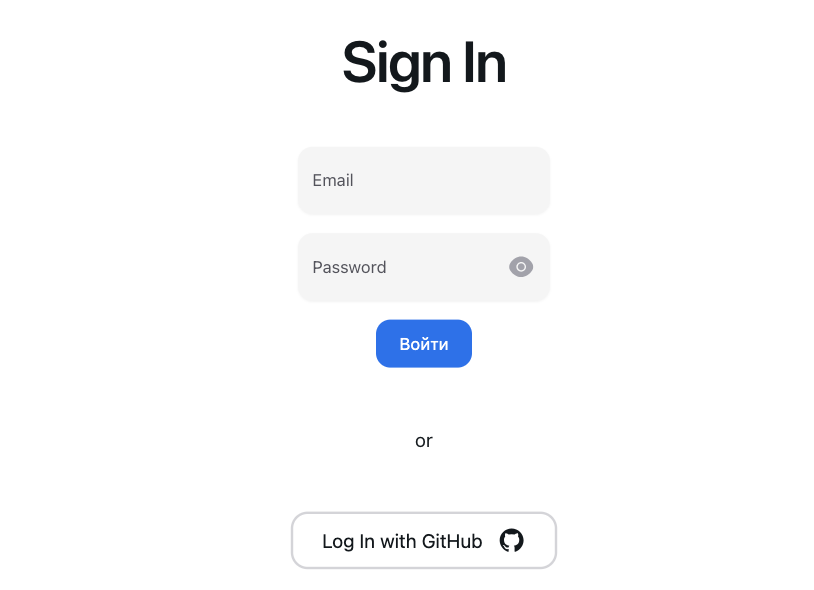
\includegraphics[width=12cm]{images/image-signin.png}
    \caption{\label{fig:1}%
        Страница авторизации}
\end{figure}




\subsection{Реализация страницы резюме}
Для написания модуля необходимо создать структуру данных резюме. Информация о профиле хранится в формате текстовом формате обмена данными JSON и содержит в себе следующие поля:
\begin{enumerate}
    \item Id -- генерируемый уникальный идентификатор резюме;
    \item Name -- фамилия и имя человека;
    \item Description -- краткое описание профиля;
    \item Social links -- ссылки на социальные сети;
    \item Profile image -- изображение работника для резюме;
    \item About -- текстовое поле с рассказом о себе, являющееся аналогом сопроводительного письма;
    \item Education, experience -- группы образования и опыта работы, включающие в себя следующие пункты:
    \begin{enumerate}
        \item Name -- наименование места работы или учебного учереждения;
        \item Description -- описание чем занимался соискатель в данное время;
        \item Start date, end date -- дата начала и окончания; 
        \item Current date -- поле, показывающее что дата окончания отсутвует и при подсчёте её следует считать текущим днём;
    \end{enumerate}
    \item Projects -- поле проектов, следующее из опыта работы. Включает в себя:
    \begin{enumerate}
        \item Name -- наименование проекта;
        \item Description -- описание проекта и над чем происходила работа;
        \item Image -- изображение проекта, его логотип, интерфейс.
    \end{enumerate}
\end{enumerate}

Последовательно реализуем компоненты, начиная с блока контактов и ссылок на социальные сети, получающий на вход список адресов и возвращающий горизонтальный список кнопок с переходом и миниатюрами соответвующих сервисов. Изображения предварительно описываются в формате svg в компоненте icons.tsx, после чего из строки выделяется имя хостинга с последующим добавлением в массив элементов для отображения на странице.
\begin{minted}[fontsize=\small, breaklines=true, style=bw, linenos]{text}
function IconVariant(service: string, icon_color:string, icon_size:number) {
switch(service) { 
    case "github.com": 
        { return <GithubIcon className={icon_color} size={icon_size}/>; } 
    default: 
        { return <InternetIcon className={icon_color} size={icon_size}/>; }
}};
export const SocialLink = (props : SocialProps) => {
    const icon_size, icon_color = 36, "text-default-500";
    const social_icons = props.links.map((element, index) => {
    var url = new URL(element.toString());
return 	
    <Link isExternal href={element.toString()} key={index}>
        {IconVariant(url.host.toString(), icon_color, icon_size)}
    </Link>;
});};
\end{minted}

Итоговый вид компонента показан на рисунке~\ref{fig:2}. 
\begin{figure}[!ht]
    \centering
    
\includegraphics[width=12cm]{images/image-resume-1.png}
    \caption{\label{fig:2}%
        Компонент отображения контактов и ссылок}
\end{figure}




Опишем компонент вывода образования и опыта работы. Для этого 
\begin{minted}[fontsize=\small, breaklines=true, style=bw, linenos]{ts}
function diffDates(day_one:any, day_two:any) {
    return (day_one - day_two) / (60 * 60 * 24 * 1000);
};
function getFormatedStringFromDays(numberOfDays:number) {
    numberOfDays = Math.abs(numberOfDays)
    var years = Math.floor(numberOfDays / 365);
    var months = Math.floor(numberOfDays % 365 / 30);
    var yearsDisplay = years > 0 ? 
        years + (years == 1 ? " year " : " years ") : "";
    var monthsDisplay = months > 0 ? 
        months + (months == 1 ? " month " : " months ") : "";
    return yearsDisplay + monthsDisplay; 
};
export const Experience = (props : ExperienceProps) => {
    const experience_item_list = props.experience_list.map((element, index)=>{
        const date1 = new Date(element.start_date);
        const date2 = element.current_date ? 
            new Date() : new Date(element.end_date)
        return { getFormatedStringFromDays(diffDates(date1, date2)) } 
    })
    return  <>{experience_item_list}</>
};
\end{minted}

Итоговый вид компонента показан на рисунке~\ref{fig:3}.  
\begin{figure}[!ht]
    \centering
    
\includegraphics[width=12cm]{images/image-resume-2.png}
    \caption{\label{fig:3}%
        Страница обновления навыков на плотформе hh.ru}
\end{figure}




Компонент проектов, выводящий шахматную структуру 
\begin{minted}[fontsize=\small, breaklines=true, style=bw, linenos]{ts}
export const Projects = (props : ProjectsProps) => {
    const projects = props.projects_list.map((element, index) => {
        var position_image = index % 2 == 0 ? "col-start-7 col-end-13" : "col-start-1 col-span-6 ";
        var position_text = index % 2 == 0 ? "col-start-1 col-end-6" : "col-start-8 col-end-13 order-1";

        return (
            <div className="grid grid-cols-12 gap-2 mb-12" key={index}>
                <div className={position_text + " h-full flex flex-col justify-center"}>
                    <h2 className="h6 uppercase text-start pb-4" id="projects">{element.name}</h2>
                    <p className="text-start">{element.description}</p>
                </div>
                <div className={position_image}>
                    <Image/>
                </div>
            </div>
        )
    })

    return  <>{projects}</>
};
\end{minted}


Итоговый вид компонента показан на рисунке 
\begin{figure}[!ht]
    \centering
    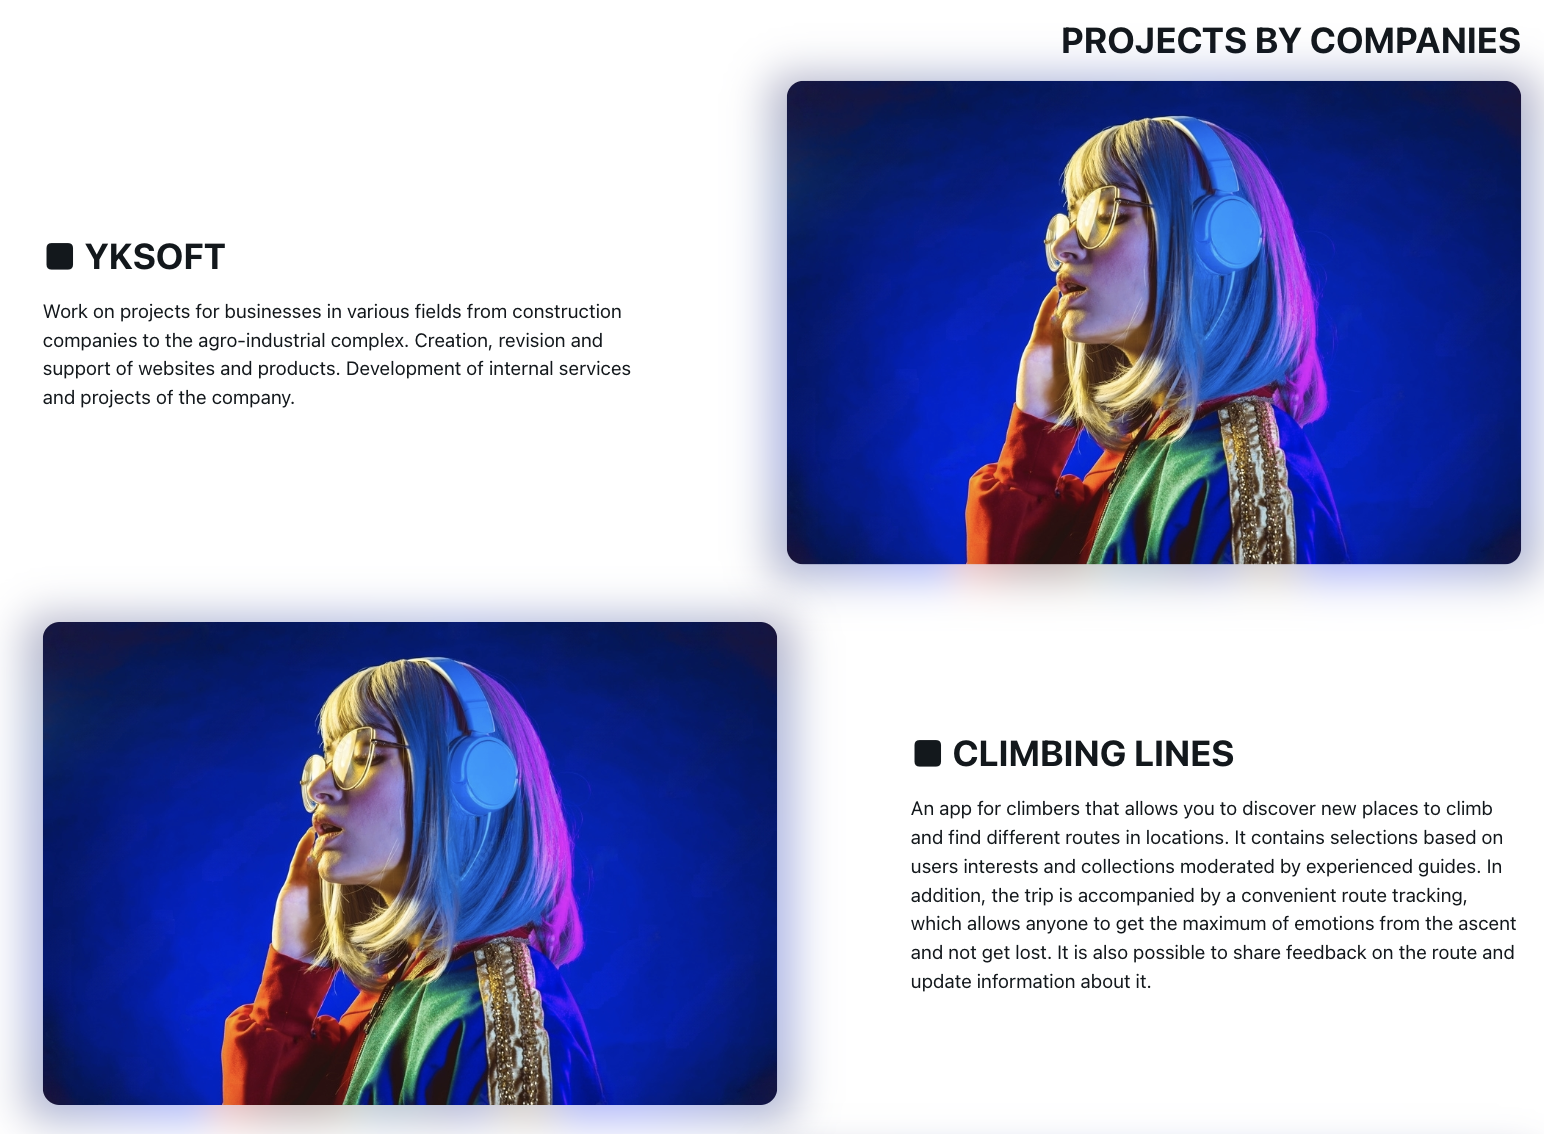
\includegraphics[width=12cm]{images/image-resume-3.png}
    \caption{\label{fig:4}%
        Страница обновления навыков на плотформе hh.ru}
\end{figure}


Произведём запрос данных у сервера и отобразим их в описанных ранее компонентах, передав в них  
\begin{minted}[fontsize=\small, breaklines=true, style=bw, linenos]{ts}
export default function Template1Page() {
    const profile_data = require("@/data-template/template-1-data.json");
	return (
		<div>
			<h1 className="h6 text-uppercase text-center pb-4">
                {profile_data.name}
            </h1>
            <p className="text-uppercase text-center pb-2">
                {profile_data.description}
            </p>
            <SocialLink links = {profile_data.social_links}/>
            <div className="grid grid-cols-8 gap-4 mb-12">
                <div className="col-start-3 col-end-7">
                    <Image
                        isZoomed
                        isBlurred
                        alt={profile_data.name + " Image"}
                        src={profile_data.profile_image}
                    />
                </div>
            </div>
			<div className="container pt-5 pb-5 text-left">
				<h2 className="h6 uppercase text-end pb-4" id="about">about me</h2>
                <About about_text={...profile_data.about}/>
    		</div>
            <div className="container pt-5 pb-5 text-left ">
                <h2 className="h6 uppercase text-end pb-4" id="experience">education</h2>
                <Experience experience_list={...profile_data.education}/>
            </div>
            <div className="container pt-5 pb-5 text-left ">
                <h2 className="h6 uppercase text-end pb-4" id="experience">experience</h2>
                <Experience experience_list={...profile_data.experience}/>
            </div>
            <div className="container pt-5 pb-5">
                <h2 className="h6 uppercase text-end pb-4" id="projects">projects by companies</h2>
                <Projects projects_list={...profile_data.projects}/>
            </div>

	    </div>
	);
}    
\end{minted}




\subsection{HH}
Процесс авторизации пользователя через hh.ru представляет из себя 3 ступени:
\begin{enumerate}
    \item Перенаправление пользователя по адресу, с переданными параметрами приложения
    \item Получение временного кода авторизации
    \item Получение токена, кода доступа к API и кода обновления  
\end{enumerate}


В api/hh/route.tsx опишем получение токена авторизации и если он есть, получения резюме
\begin{minted}[fontsize=\small, breaklines=true, style=bw, linenos]{ts}
export async function GET(req: Request) {

const { searchParams } = new URL(req.url)
const code = searchParams.get('code');
const token = searchParams.get('token');


if (code != null) {
    var myHeaders = new Headers();
    myHeaders.append("Content-Type", "application/x-www-form-urlencoded");

    var urlencoded = new URLSearchParams();
    urlencoded.append("grant_type", "authorization_code");
    urlencoded.append("client_id", process.env.HH_ID!);
    urlencoded.append("client_secret", process.env.HH_SECRET!);
    urlencoded.append("code", code!);

    try {
        const res = await fetch("https://hh.ru/oauth/token", {
            method: 'POST',
            headers: myHeaders,
            body: urlencoded,
            redirect: 'follow',
        });
            
        const result = await res.json();
        return NextResponse.json(result);
    } 
    catch (error) {
        console.log(error);
    }
} 


if (token != null) {
    var myHeaders = new Headers();
    myHeaders.append("Authorization", `Bearer ${token}`);

    try {
        const res = await fetch("https://api.hh.ru/resumes/mine", {
            method: 'GET',
            headers: myHeaders,
            redirect: 'follow',
        });
            
        const result = await res.json();
        return NextResponse.json(result);
    } 
    catch (error) {
        console.log(error);
    }
}
return NextResponse.json("bad request");
}
\end{minted}



В api/hh/route.tsx опишем обновление резюме
\begin{minted}[fontsize=\small, breaklines=true, style=bw, linenos]{ts}
export async function PUT(req: Request) {
    const { searchParams } = new URL(req.url)
    const resume = searchParams.get('resume');

    if (resume != null) {
        const body = await req.json()
        
        var myHeaders = new Headers();
        myHeaders.append("User-Agent", process.env.HH_APP_DATA!);
        myHeaders.append("Content-Type", "application/json");
        myHeaders.append("Authorization", `Bearer ${process.env.HH_USER}`);

        var raw = JSON.stringify( body );

        try {
            const res = await fetch(`https://api.hh.ru/resumes/${resume}`, {
                method: 'PUT',
                headers: myHeaders,
                body: raw,
                redirect: 'follow'
            })
            return NextResponse.json({ message: "Resume has been updated" });
        } 
        catch (error) {
            console.log(error);
            return NextResponse.json({ message: error });
        }
    }  
}
\end{minted}



Для взаимодействия с апи между клиентской и серверной частью опишем методы getUserResume и 
getUserToken, получающие токен и код данных
\begin{minted}[fontsize=\small, breaklines=true, style=bw, linenos]{ts}
export async function getUserResume(token: string) {
	try {
		const response = await fetch('/api/hh?token=' + token);
		const data = await response.json();

		if (!data.error) {
			return data.access_token;
		} else {
			return data.error;
		}
		
	} catch (error){
		console.log(error);
	}
}
\end{minted}


И теперь опишем страницу авторизации через hh
\begin{minted}[fontsize=\small, breaklines=true, style=bw, linenos]{text}
export default function HHSignInPage() {

const searchParams = useSearchParams()
const code = searchParams.get('code')

const [url, setUrl] = React.useState('')
React.useEffect(() => {
    getDownloadURL().then(setUrl)
}, [])
async function getDownloadURL(){
    const resultData = getUserToken(code!);
    return await Promise.resolve(resultData)
}
return (
    <section className="flex flex-col items-center justify-center gap-24 ">
        <h1>HH Sign In Page</h1>

        <div className="flex flex-col items-center justify-center gap-2">
            SignIn Token:
            <Code size="lg">{code}</Code>
        </div>
        
        <div className="flex flex-col items-center justify-center gap-2">
            Access Token:
            <Suspense fallback={<div>Loading...</div>}>
                <Code size="lg">{url}</Code>
                <p className="opacity-60 mb-24">Сохраните токен из поля выше для дальнейшей работы с сайтом</p>

                <Link isExternal href={'/api/hh?token=' + url}>
                    <Button>Посмотреть мои резюме</Button>
                </Link>

            </Suspense>
        </div>

    
    </section>
);
}   
\end{minted}


\subsection{Страница сравнения навыков}
Для страницы сравнения навыков реализуем компонент строки, принимающей строку данных
\begin{minted}[fontsize=\small, breaklines=true, style=bw, linenos]{ts}
export const ActionFieldButton = () => {
    return (
        <div className="flex gap-4 items-center">
            <Button color="success" variant="bordered">
                Add item
            </Button>    
            <Button color="danger" variant="bordered" className="min-w-0">
                <DeleteIcon/>
            </Button>
        </div>
    )
}

export const Comparison = (props: ComparisonItemProps) => {
    

    let cv_editor_item_list;
    if (typeof props.cv_editor == "string") {
        cv_editor_item_list = <div>{props.cv_editor}</div>;
    } else {
        Object.keys(props.cv_editor).map((element, index) => {
            let arrObj = props.cv_editor[element];
            if (typeof arrObj == "object") {
                cv_editor_item_list = props.cv_editor.map((element: any, index:any) => {
                    return (
                        <div key={index}>
                            {Object.keys(element).map((el, index) => {
                                return( 
                                    <div key={index}>
                                        <span className="font-bold opacity-40">{el}: </span>{element[el]}
                                    </div> 
                                );
                            })}
                            <Spacer y={4} />
                        </div>
                    );
                });  
            } else {
                cv_editor_item_list = props.cv_editor.map((element: any, index:any) => {
                    return (
                        <div key={index}>
                            {element}
                            <Spacer y={2} />
                        </div>
                    );
                })
            }
        });
    }


    let hh_ru_item_list;
    if (typeof props.hh_ru == "string") {
        hh_ru_item_list = <div>{props.hh_ru}</div>;
    } else {
        Object.keys(props.hh_ru).map((element, index) => {
            let arrObj = props.hh_ru[element];
            if (typeof arrObj == "object") {
                hh_ru_item_list = props.hh_ru.map((element: any, index:any) => {
                    return (
                        <div key={index}>
                            {Object.keys(element).map((el, index) => {
                                return( 
                                    <div key={index}>
                                        <span className="font-bold opacity-40">{el}: </span>{element[el]}
                                    </div> 
                                );
                            })}
                            <Spacer y={4} />
                        </div>
                    );
                });  
            } else {
                hh_ru_item_list = props.hh_ru.map((element: any, index:any) => {
                    return (
                        <div key={index}>
                            {element}
                            <Spacer y={2} />
                        </div>
                    );
                })
            }
        });
    }



    return  (
        <section className="">        
            <Divider className="my-8" />

            <RadioGroup orientation="horizontal" defaultValue="answer-1" className="flex gap-2 mb-4 text-start ">     
                <div className="w-1/6 items-start font-bold opacity-80">
                    {props.name}
                </div>
                <Radio value="answer-1" className="w-2/6 max-w-full items-start">
                    {cv_editor_item_list}
                </Radio>
                <Radio value="answer-2" className="w-2/6 max-w-full items-start">
                    {hh_ru_item_list}
                </Radio>
                <Radio value="answer-3" className="w-1/6 max-w-full items-start">
                    <ActionFieldButton />
                </Radio>  
            </RadioGroup>
  
        </section>

    )};    
\end{minted}

\begin{figure}[!ht]
    \centering
    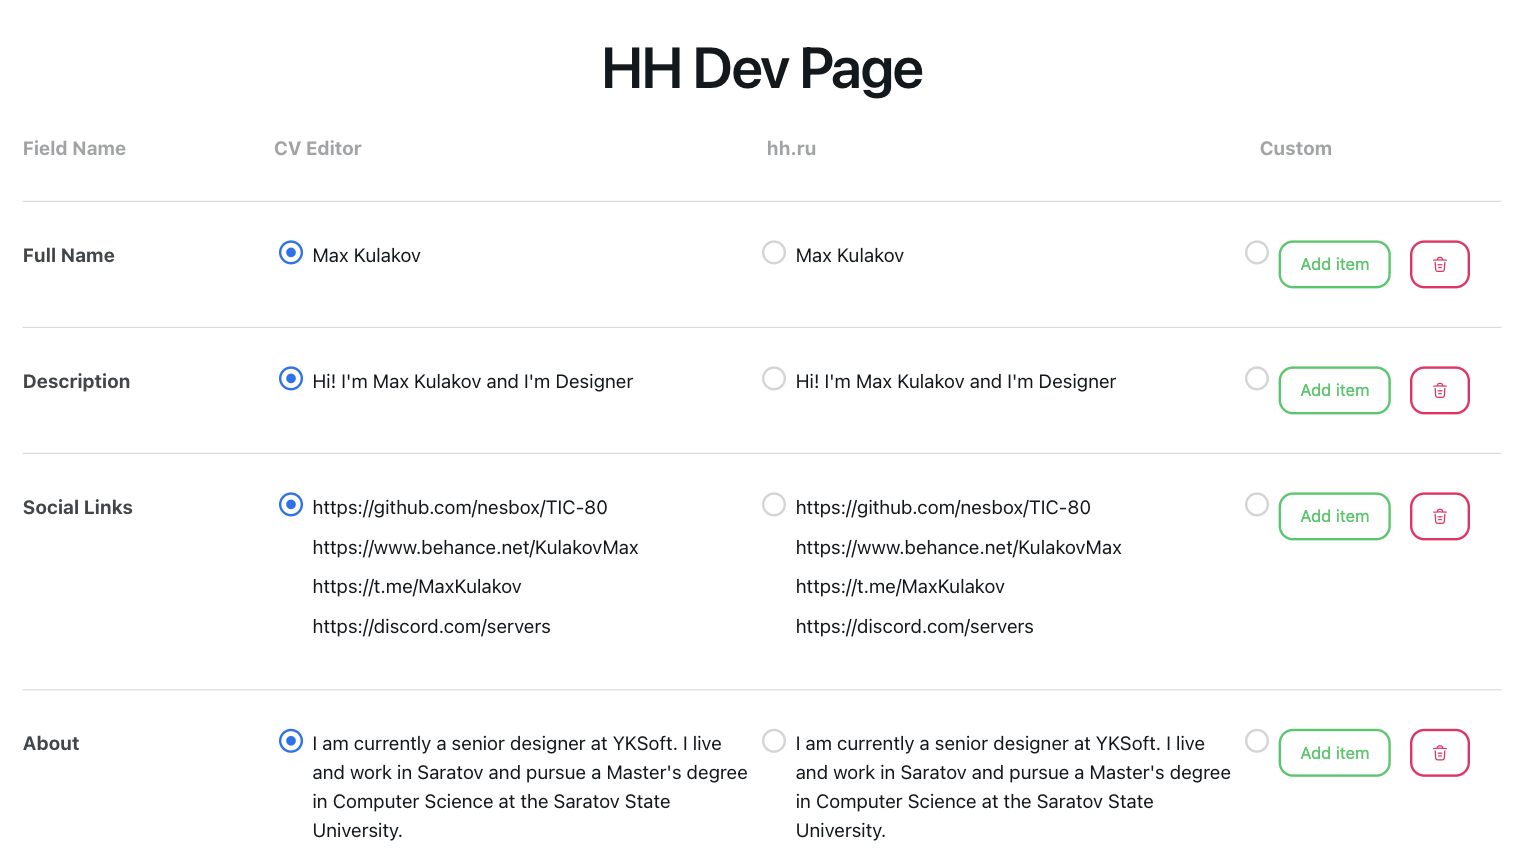
\includegraphics[width=12cm]{images/image-compare-skills.png}
    \caption{\label{fig:5}%
        Страница сравнения навыков}
\end{figure}




\subsection{Страница обновления навыков}
Для страницы обновления навыков обратимся к ранее описанному апи
\begin{minted}[fontsize=\small, breaklines=true, style=bw, linenos]{ts}
export default function ResumePage() {
	
	const session = useSession();
	const profile_data = require("@/data-template/template-hh-data.json");

	const initialSkills = profile_data.skill_set
	const [skill_set, setSkill_set] = React.useState(initialSkills);
	
	const handleClose = (skillToRemove:any) => {
		setSkill_set(skill_set.filter((fruit: any) => fruit !== skillToRemove));
		if (skill_set.length === 1) {
		  setSkill_set(initialSkills);
		}
	};

	const skills_body = JSON.parse(JSON.stringify(`{"skill_set": [${skill_set.map((x: any) => `"${x}"`)}]}`))
	function updateResume() {
		const postData = async () => {

			const response = await fetch("/api/hh?resume=986544fbff0b05dce60039ed1f53716830586e", {
				method: "PUT",
				body: skills_body,
			});
			console.log(skills_body);
			return response.json();
		};
		postData().then((data) => {
			console.log(data.message);
		});
	}

	const [inputValue, setInputValue] = React.useState("");


	return (
		<section className="flex flex-col items-center justify-center gap-24">
			<h1 className={title()}>Резюме HH.ru</h1>



			<div className="">
				<h2 className="mb-4">	
					Навыки 
					<span className="opacity-100">
						{skill_set == initialSkills? 
						<div className="text-green-600"> [ не изменено ]</div> 
						: 
						<div className="text-yellow-600"> [ изменено ]</div>}
					</span>
				</h2>
				<div className="flex flex-wrap gap-2">
					{skill_set.map((skill: any, index: any) => (
						<Chip key={index} onClose={() => handleClose(skill)} variant="flat">
							{skill}
						</Chip>
					))}
				</div>
			</div>

			<div className="w-full flex flex-col gap-2 items-center justify-center max-w-[640px]">
				<Input
					label="Skill"
					placeholder="Add skill to pool"
					value={inputValue}
					onValueChange={setInputValue}
				/>
				<Button 
					className="max-w-[240px]"
					onClick={() => { setSkill_set([...skill_set, inputValue]); }}
				>
					Добавить навык
				</Button>
			</div>
			
			<Button onClick={updateResume}>Обновить резюме</Button>
			

		</section>
	);
}
\end{minted}


Итоговый вид страницы обновления навыков представлен на рисунке~\ref{fig:1} 
\begin{figure}[!ht]
    \centering
    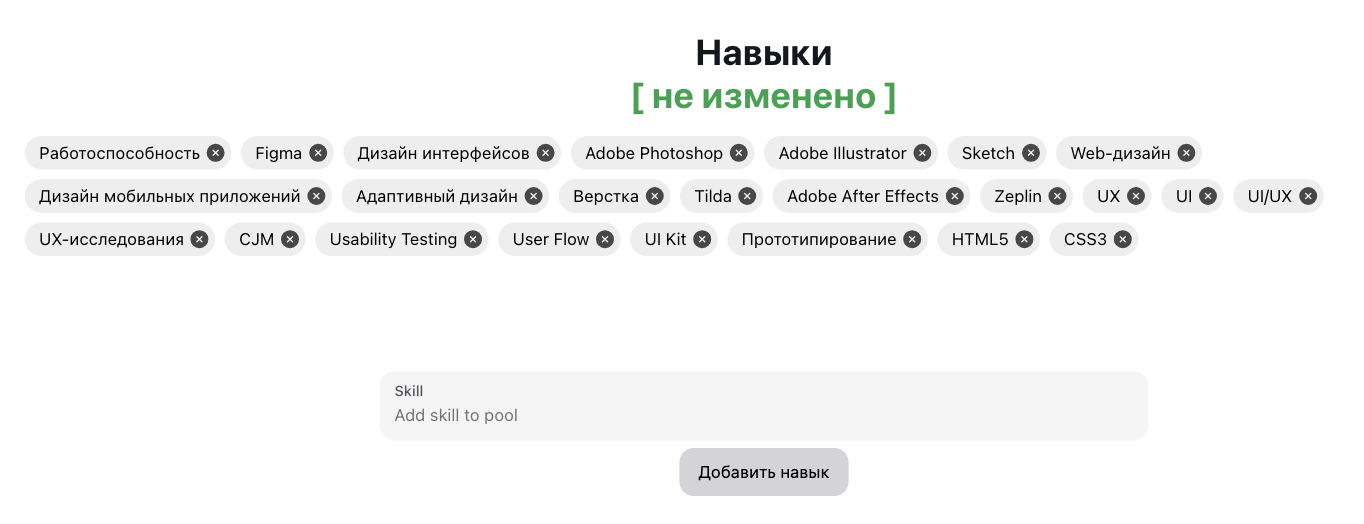
\includegraphics[width=12cm]{images/image-update-skills.png}
    \caption{\label{fig:6}%
        Страница обновления навыков на плотформе hh.ru}
\end{figure}







\newpage
\conclusion
В результате проведения исследовательской работы были приобретены навыки анализа 
качества и эффективности научной литературы в области разработки сервисов 
с автоматическим обновлением данных, достигнут навык анализирования конкурентных 
платформ для создания резюме и сформулирован собственный метод разработки 
единой платформы резюме, тем самым было достигнуто полное выполнение поставленных задач.

В качестве объектов анализа научной литературы выступили статьи по темам составления 
резюме, их анализа со стороны социологии, а также статьи, в которых рассматриваются 
инструменты для веб-разработки. С учётом проведённого анализа научной литературы 
были составлены основные требования для разработки будущей платформы как с технической 
стороны, так и со стороны гуманитарно-социальных наук.

Анализ конкурентных платформ позволил выявить слабые стороны существующих сервисов, 
исправление которых возможно реализовать в разработке собственной единой платформы 
резюме при условии его дальнейшего масштабирования. \cite{Arhipov_2015}




% Библиографический список, составленный вручную, без использования BibTeX
%
% \begin{thebibliography}{99}
%   \bibitem{Ione} Источник 1.
%   \bibitem{Itwo} Источник 2
% \end{thebibliography}

% Отобразить все источники. Даже те, на которые нет ссылок.
% \nocite{*}

% Меняем inputencoding на лету, чтобы работать с библиографией в кодировке
% `cp1251', в то время как остальной документ находится в кодировке `utf8'
\inputencoding{cp1251}
\bibliographystyle{gost780uv}
\bibliography{thesis}
\inputencoding{utf8}



% При использовании biblatex вместо bibtex
% \printbibliography

% Окончание основного документа и начало приложений Каждая последующая секция
% документа будет являться приложением
\appendix


\section{Код Компонента}
Да


\end{document}
